\begin{figure*}
\centering
\begin{subfigure}[t]{0.475\textwidth}
\begin{tikzpicture}[thick, scale=0.7, every label/.style={align=left, scale=0.7}]
   \pie[text=legend, sum=auto, hide number, color={blue!60, cyan!60, yellow!60}]{
      20/46.5\%,
      18/41.9\%,
      5/11.6\%
}
\end{tikzpicture}
\caption{Discrepancies found in standards.}
\label{fig:stdDiscrepSources}
\end{subfigure}
\hfill
\begin{subfigure}[t]{0.475\textwidth}
\begin{tikzpicture}[thick, scale=0.7, every label/.style={align=left, scale=0.7}]
   \pie[text=legend, sum=auto, hide number, color={blue!60, yellow!60, orange!60}]{
      19/36.5\%,
      25/48.1\%,
      8/15.4\%
}
\end{tikzpicture}
\caption{Discrepancies found in ``meta-level''\\documents.}
\label{fig:metaDiscrepSources}
\end{subfigure}
\vskip\baselineskip
\begin{subfigure}[t]{0.475\textwidth}
\begin{tikzpicture}[thick, scale=0.7, every label/.style={align=left, scale=0.7}]
   \pie[text=legend, sum=auto, hide number, color={blue!60, yellow!60, orange!60, red!60}]{
      6/35.3\%,
      6/35.3\%,
      4/23.5\%,
      1/5.9\%
}
\end{tikzpicture}
\caption{Discrepancies found in textbooks.}
\label{fig:textDiscrepSources}
\end{subfigure}
\hfill
\begin{subfigure}[t]{0.475\textwidth}
\begin{tikzpicture}[thick, scale=0.7, every label/.style={align=left, scale=0.7}]
   \pie[text=legend, sum=auto, hide number, color={blue!60, yellow!60, orange!60, red!60, blue!60!cyan!60}]{
      11/22.4\%,
      20/40.8\%,
      14/28.6\%,
      1/2\%,
      3/6.1\%
}
\end{tikzpicture}
\caption{Discrepancies found in other\\documents.}
\label{fig:otherDiscrepSources}
\end{subfigure}
\vskip\baselineskip
\begin{center}
\begin{subfigure}[t]{\linewidth}
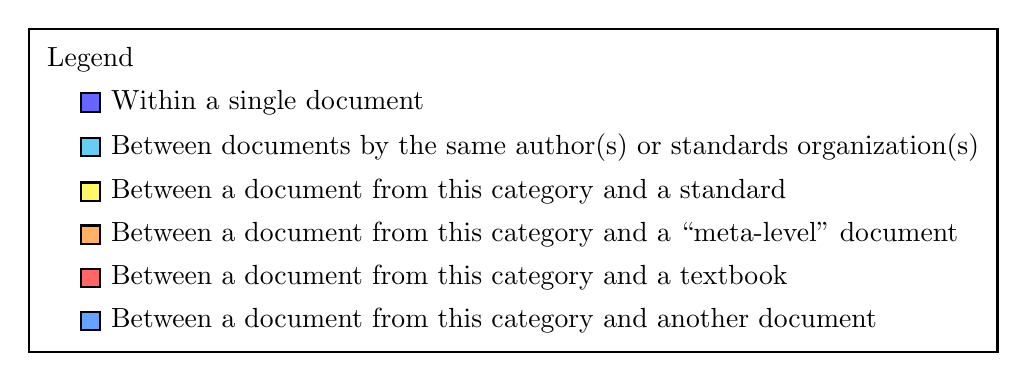
\begin{tikzpicture}
\matrix [thick, draw=black] {
\node[label=center:Legend] {{}}; \\
\node[thick, shape=rectangle, draw=black, fill=blue!60, label=right:{Within a single document}](0) {}; \\
\node[thick, shape=rectangle, draw=black, fill=cyan!60, label=right:{Between documents by the same author(s) or standards organization(s)}](1) {}; \\
\node[thick, shape=rectangle, draw=black, fill=yellow!60, label=right:{Between a document from this category and a standard}](2) {}; \\
\node[thick, shape=rectangle, draw=black, fill=orange!60, label=right:{Between a document from this category and a ``meta-level'' document}](3) {}; \\
\node[thick, shape=rectangle, draw=black, fill=red!60, label=right:{Between a document from this category and a textbook}](4) {}; \\
\node[thick, shape=rectangle, draw=black, fill=blue!60!cyan!60, label=right:{Between a document from this category and another document}](5) {}; \\
};
\end{tikzpicture}
\end{subfigure}
\end{center}
\hfill
\caption{Sources of discrepancies based on \hyperref[sources]{source category}.}
\label{fig:discrepSources}
\end{figure*}
